% vim: ts=2 et
\chapter{Kinematics}

% --------------------------------------------- %

\section{Why vorticity is half of angular velocity?}


But why the definition of vorticity is half of angular velocity?
It is basically the definition of vorticity. Take that as a fluid particle.
The vorticity \(\omega\) is defined as twice the average angular velocity \(\Omega\) of the angular deformation.
As you can see in the picture, if the fluid particle is actually undeformable (rigid rotation), you'll always have \(\d\alpha = \d\beta\), which implies that both angular velocities of deformation are equal, thus \(\d\alpha = \d\beta = \d\theta\)
and thus \(\omega = 2 \Omega = 2\, \nf{1}{2}\left(\nf{\d \theta}{\d t} + \nf{\d \theta}{\d t} \right) = 2\, \nf{\d \theta}{\d t}\).
Vorticity is actually a definition for mathematical beauty, removing the factor two out of equations, because, generally, the average angular velocity will be \(\nf{1}{2} \left(\nf{\d \alpha}{\d t} + \nf{\d \beta}{\d t}\right)\) \cite{quoraHobold}.



% --------------------------------------------- %

\section{Fluid Element Kinematics}


In fluid mechanics (as in solid mechanics), an element may undergo four fundamental types of motion: translation, rotation, linear strain, and shear strain, shown in the~\cref{fig:fluid-element-types-of-transormations}.
%
\begin{figure}[H]
  \centering
  \incfig{fluid-element-types-of-transormations}
  \caption{Four types of transformation that a fluid element can experience. A fluid element at time \(t\) is shown in a gray square with a solid border, and the fluid element after transformation at time \(t + \d t\) is represented with a transparent gray square with a dashed border.}
  \label{fig:fluid-element-types-of-transormations}
\end{figure}
%
Because fluids are in constant motion, motion and deformation is best described in terms of rates:
%
\begin{itemize}
  \item velocity: rate of translation
  \item angular velocity : rate of rotation
  \item shear strain rate: rate of shear strain
  \item linear strain rate: rate of linear strain
\end{itemize}
%
\begin{figure}[H]
  \centering
  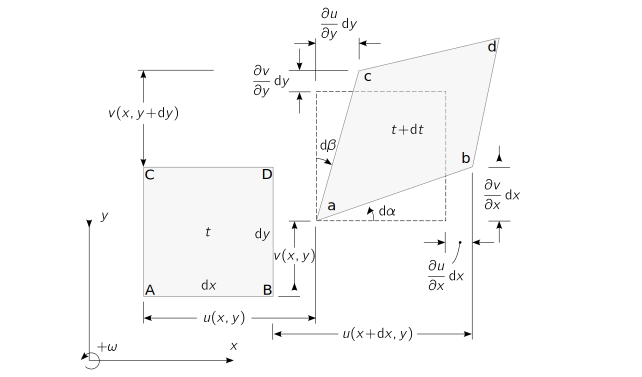
\includegraphics[width=\linewidth]{fluid-element-deformation}
  \caption{Fluid Element Deformation.}
  \label{fig:fluid-element-deformation}
\end{figure}
%
To be useful, these deformation rates must be expressed in terms of velocity and derivatives of velocity.
During infinitesimal time period \(\d t\), the rectangular fluid element can deform in four ways~(\cref{fig:fluid-element-deformation}):
%
\begin{enumerate}
  \item \textbf{Rigid body linear motion.}\quad
    %
    The \textbf{rate of translation vector} is described mathematically as the velocity vector.
    In Cartesian coordinates: \(\U = u \mathrm{\mb{i}} + v \mathrm{\mb{j}} + w \mathrm{\mb{k}}\).
    It disappears when \(\U = 0\).

  \item \textbf{Rigid body rotation.}\quad
    %
    \textbf{Rate of rotation} (angular velocity [\si{\nf{\text{radians}}{\s}}]), \(\nf{\d\mbg{\Omega}}{\d t}\), at a point is defined as the average rotation rate of two lines which are initially perpendicular and that intersect at that point~\cite{courseUniGeBottaro}.
      In other words, it is the ratio of change in angular rotation divided by the time period through which rotation was done.
      As there are two lines that are rotating, AB and AC, for a measure of change in angle of the element, we compute the average of these two angles.
        By convention, the counter-clockwise rotation is considered positive and vice versa.
        For an element in the \(xy\)-plane, the mean angular rotation about the \(z\)-axis at point A is
        %
        \begin{equation}
          \d \Omega_z = \f{1}{2} \left(\d \alpha + \d \beta\right),
          \label{eq:angular-rotation}
        \end{equation}
        %
        in which
        %
        \begin{equation}
          % NOTE: first argument to underbrace is display style. The second argument is in text style.
          % To have any part of the first argument in textstyle (e.g. the case of a frac inside of
          % another frac) use \textstyle
          \begin{aligned}
            \d \alpha & = \lim_{\d t \to 0} \Biggl(\tan^{-1}\f{\ddx{v} \bcancel{\d x} \d t}{\bcancel{\d x} + \underbrace{{\textstyle\ddx{u}} \bcancel{\d x} \d t}_{\to 0}} \Biggr) = \ddx{v} \d t, \\
            %
            \d \beta  & = \smallunderbrace{\mathclap{-}}_{\substack{\clap{\text{\tiny CW}}\\\clap{\text{\tiny rotation}}}} \lim_{\d t \to 0} \Biggl(\tan^{-1}\f{\ddx{u} \bcancel{\d y} \d t}{\bcancel{\d y} + \underbrace{{\textstyle\ddx{v}} \bcancel{\d y} \d t}_{\to 0}} \Biggr) = -\ddy{u} \d t.
          \end{aligned}
          \label{eq:differential-angles}
        \end{equation}
        %
        This type of motion is absent when \(\d\alpha = \d\beta\) (distortion without rotation).
        Two other components \(\Omega_z\) and \(\Omega_y\) can be computed in a similar manner.
        So, the angular velocity components in three directions equal~\cite{ghazanfarian2024applied}
        %
        \begin{equation}
          \begin{aligned}
            \ddt{\Omega_z} &= \f{1}{2} \left(\ddx{v} - \ddy{u}\right), \\
            \ddt{\Omega_x} &= \f{1}{2} \left(\ddy{w} - \ddz{v}\right), \\
            \ddt{\Omega_y} &= \f{1}{2} \left(\ddz{u} - \ddx{w}\right).
        \end{aligned}
          \label{eq:angular-velocity-components}
        \end{equation}
        %
        In vector notation
        \begin{equation}
          \ddt{\mbg{\Omega}} = \f{1}{2} \grad\times\U.
          \label{eq:angular-velocity-vector-notation}
        \end{equation}
        %
        The curl of the velocity field is called \emph{vorticity}, \(\mbg{\omega}\), thus,
        %
        \begin{equation}
          \ddt{\mbg{\Omega}} = \f{1}{2} \mbg{\omega}
          \label{eq:vorticity-and-angular-velocity}
        \end{equation}
        %
  \item \textbf{The dilation\footnote{Dilatation is also correct} or the extensional strain-rate}.\quad
    \textbf{Linear strain} is defined as the rate of change in length per unit length~\cite{courseUniGeBottaro}.
    \textbf{Linear strain rate} is the change of linear strain of the material with respect to time.
    Another way to express it would be the (temporal) rate at which the distance between two parallel sides of the element change~\cite{ghazanfarian2024applied}.
    Linear strain (rate) is calculated as the change in dimension \(\Delta L\) divided by the original dimension \(L\).
    In the \(x\)-direction:
    %
    \begin{equation}
      \begin{aligned}
      &\epsilon_{xx} \d t = \f{\Delta L}{L} = \f{\left(\d x + \ddx{u} \d x \d t\right) - \d x}{\d x} = \ddx{u} \d t \\
        \implies\quad &\epsilon_{xx} = \ddx{u}.
      \end{aligned}
      \label{eq:linear-strain-x-direction}
    \end{equation}
    %
    Similarly for other directions
    %
    \begin{equation}
      \begin{aligned}
        \epsilon_{yy} &= \ddy{v} \\
        \epsilon_{zz} &= \ddz{w}
      \end{aligned}
      \label{eq:linear-strain-rate-y-and-z-direction}
    \end{equation}

    The rate of increase of volume of a fluid element per unit volume is the \textbf{volumetric strain rate}, in Cartesian coordinates.
    For the case of incompressible flow, since the volume of a fluid element is constant, the volumetric strain rate must be zero.
    %
  \item \textbf{The shear or the distortional shear strain-rate}.\quad
    Shear strain rate at a point is defined as half the rate of decrease of the angle between two initially perpendicular lines (AB and AC) that intersect at a point (A)~\cite{courseUniGeBottaro}.
    In the \(xy\)-plane
    %
    \begin{equation}
      \epsilon_{xy} \d t = \f{1}{2} \left(\d \alpha - \d \beta\right) = \f{1}{2} \left(\ddy{u} - \left(-\ddx{v}\right)\right) \d t.
      \label{eq:shear-strain-xy-plane}
    \end{equation}
    %
    Therefore shear strain rate will be the following for \(xy\)-, \(yz\)- and \(zx\)-plane
    %
    \begin{equation}
      \begin{aligned}
        \epsilon_{xy} &= \f{1}{2} \left(\ddy{u} + \ddx{v}\right) \\
        \epsilon_{yz} &= \f{1}{2} \left(\ddy{w} + \ddz{v}\right) \\
        \epsilon_{zx} &= \f{1}{2} \left(\ddz{u} + \ddx{w}\right)
      \end{aligned}
      \label{eq:shear-strain-rate-components}
    \end{equation}
    %
    where \(\epsilon_{xy} = \epsilon_{yx}, \epsilon_{yz} = \epsilon_{zy}, \epsilon_{xz} = \epsilon_{zx}\) are the off-diagonal elements of the \emph{strain rate tensor}~\cite{ghazanfarian2024applied}.
    This type of deformation vanishes when \(\d \alpha = -\d \beta\) (rotation without distortion)~\cite{ghazanfarian2024applied}.
    From the procedure of derivation of the strain rate components, it is obvious that the strain rate tensor is symmetric \(\epsilon_{ij} = \epsilon_{ji}\)~\cite{ghazanfarian2024applied}.
    In~\cref{fig:fluid-element-deformation}, points A and D experience negative shear strain and vice versa for points B and C.
\end{enumerate}


\subsection{The strain-rate tensor} %---%

We can combine linear strain rate and shear strain rate into one \textbf{symmetric second-order} tensor called \emph{strain-rate tensor}, \(\E\)~\cite{courseUniGeBottaro}.
In Cartesian coordinates
%
\begin{equation}
  \begin{pmatrix}
    \epsilon_{xx} & \epsilon_{xy} & \epsilon_{xz} \\
    \epsilon_{yx} & \epsilon_{yy} & \epsilon_{yz} \\
    \epsilon_{zx} & \epsilon_{zy} & \epsilon_{zz}
  \end{pmatrix}
  =
  \begin{pmatrix}
    \ddx{u} & \f{1}{2}\left(\ddy{u} + \ddx{v}\right) & \f{1}{2}\left(\ddz{u} + \ddx{w}\right) \\
    \f{1}{2} \left(\ddx{v} + \ddy{u}\right) & \ddy{v} & \f{1}{2} \left(\ddz{v} + \ddy{w}\right) \\
    \f{1}{2} \left(\ddx{w} + \ddz{u}\right) & \f{1}{2}\left(\ddy{w} + \ddz{v}\right) & \ddz{w}
  \end{pmatrix}
  \label{eq:strain-rate-tensor}
\end{equation}
%
The strain-rate tensor is obtained from neither a conservation law nor a constitutive relation.
It is the fruit of a kinematic analysis of an element of the material~\cite{ghazanfarian2024applied}.

The trace of the strain-rate tensor (or its first invariant) is equal to the divergence of the velocity field.
It is the sum of three dilatations and exhibits the total rate of change of volume of the element per unit volume.
The volume change in \(x\), \(y\), \(z\) directions are \((\ddx{u}\d x \d t) \d y \d z\), \((\ddy{v}\d y \d t) \d x \d z\), and \((\ddz{w}\d z \d t) \d x \d y\), respectively.
% Then, the total rate of change of volume per volume of the differential element \((\f{1}{\d V})(\f{\D \d V}{\D t})\) is
